\documentclass{beamer}
\setbeamertemplate{navigation symbols}{}

\usepackage{beamerthemeshadow}
\usepackage{comment}
\setbeamertemplate{caption}[numbered]

\hypersetup{colorlinks}

\def\gw#1{gravitational wave#1 (GW#1)\gdef\gw{GW}}
\def\ns#1{neutron star#1 (NS#1)\gdef\ns{NS}}

\newcommand{\red}[1]{{\color{red}{#1}}}

\begin{document}
\title{BNS Windowing Examples}
\author{James A. Clark}
%\institute{Georgia Institute Of Technology}
\date{} 

\begin{frame}[plain]
\titlepage
\end{frame}

%\begin{frame}\frametitle{Table of contents}\tableofcontents
%\end{frame} 

%\section{{\tt LALSimulation} \& Burst Injections}

\begin{frame}
    \frametitle{Windowing Experiment}
    Can get good ($>90\%$ match between a \emph{simple} sine-Gaussian template and
    post-merger waveforms $\iff$ we truncate at merger (e.g., inspiral peak),
    $t_{\text{peak}}$.

    Would allow very simple and pretty robust parameter estimation to measure
    $f_{\text{peak}}$.

    Questions:
    \begin{enumerate}
        \item What happens when we try to measure $f_{\text{peak}}$ with a
            sine-Gaussian and no truncation?
        \item How accurately can we measure $t_{\text{peak}}$?
        \item \textcolor{red}{What would this truncation do to the qualitative / quantitative
            features of the spectrum?}
        \item What happens to the parameter estimation, using simple templates,
            \emph{with} truncation?
    \end{enumerate}

\end{frame}

\begin{frame}
    \frametitle{Truncation}
    Easiest to start with q.3; impact on \emph{signal} of truncation
    \begin{itemize}
        \item Following plots: blue=original waveform, red=truncated waveform.

        \item `Delay' = time, with respect to $t_{\mathrm{peak}}$, at which we
            truncate the waveform

        \item Note: truncation=chop off and then \emph{taper} waveform according
            to \url{http://arxiv.org/abs/gr-qc/0001023}

    \end{itemize}
    
\end{frame}

%
% Shen 1.35, 1.35
%
\begin{frame}
    \frametitle{Shen: 1.35-1.35: Time series / spectra}

    \begin{columns}[]
        \column{0.5\textwidth}
        \begin{center}
        \begin{figure}
            \scalebox{0.25}{
            \includegraphics{shen_135135_lessvisc-time_spec--3_15.eps}
            }
        \end{figure}
        \vspace{-0.5cm}
        \begin{figure}
            \scalebox{0.25}{
            \includegraphics{shen_135135_lessvisc-time_spec--2_75.eps}
            }
        \end{figure}
        \end{center}

        \column{0.5\textwidth}
        \begin{center}
        \begin{figure}
            %\vspace*{-0.5cm}
            \scalebox{0.25}{
            \includegraphics{shen_135135_lessvisc-time_spec--1_18.eps}
            }
        \end{figure}
        \vspace{-0.5cm}
        \begin{figure}
            \scalebox{0.25}{
            \includegraphics{shen_135135_lessvisc-time_spec-0_00.eps}
            }
        \end{figure}
        \end{center}
    \end{columns}

\end{frame}

\begin{frame}
    \frametitle{Shen: 1.35-1.35: Time series / spectra: peak trends}

    \begin{center}
        \begin{figure}
            \scalebox{0.5}{
                \includegraphics{shen_135135_lessvisc_peakfreqs.eps}
            }
        \end{figure}
    \end{center}
\end{frame}

%
% APR 1.35, 1.35
%
\begin{frame}
    \frametitle{APR: 1.35-1.35: Time series / spectra}

    \begin{columns}[]
        \column{0.5\textwidth}
        \begin{center}
        \begin{figure}
            \scalebox{0.25}{
            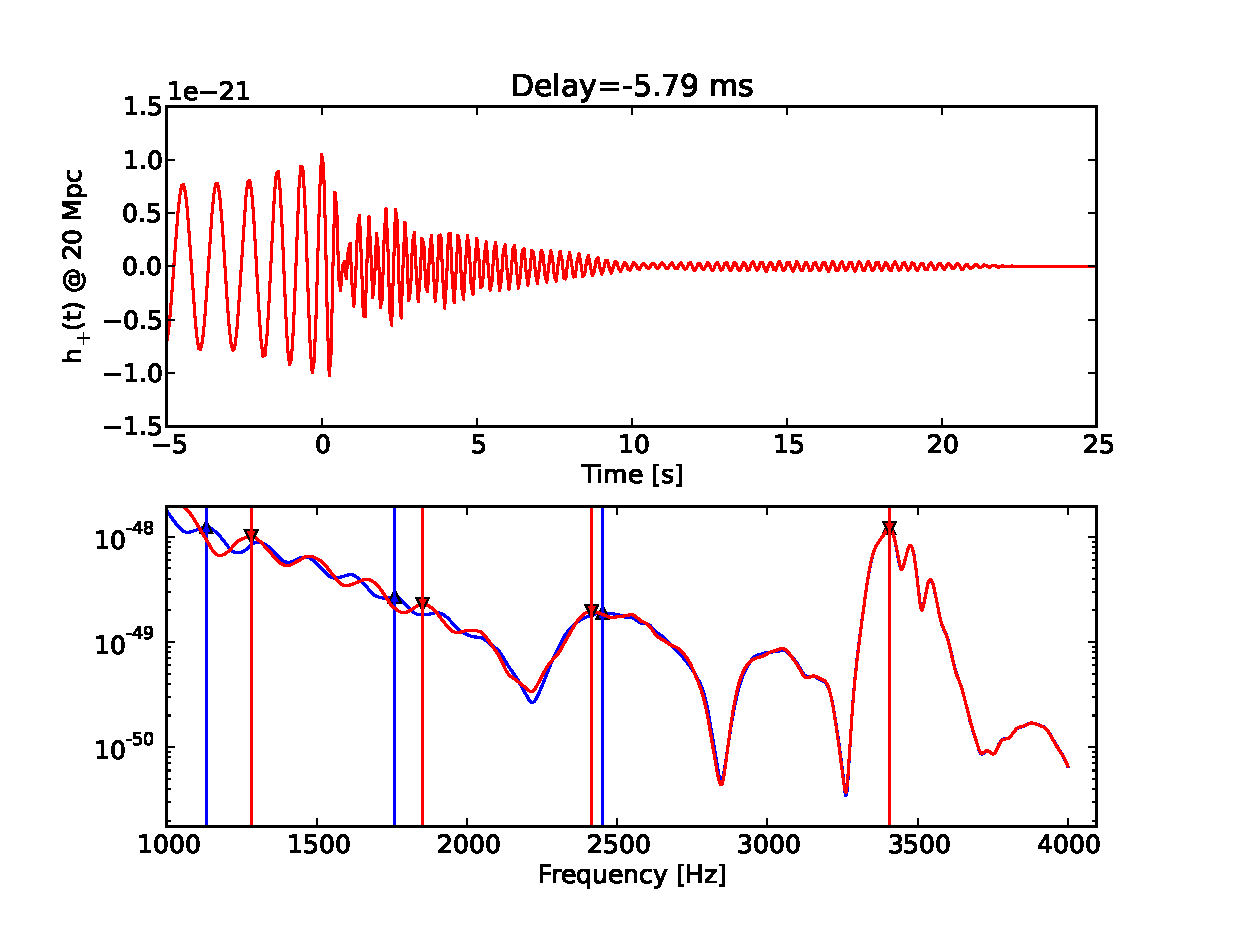
\includegraphics{apr_135135_lessvisc-time_spec--5_79.eps}
            }
        \end{figure}
        \vspace{-0.5cm}
        \begin{figure}
            \scalebox{0.25}{
            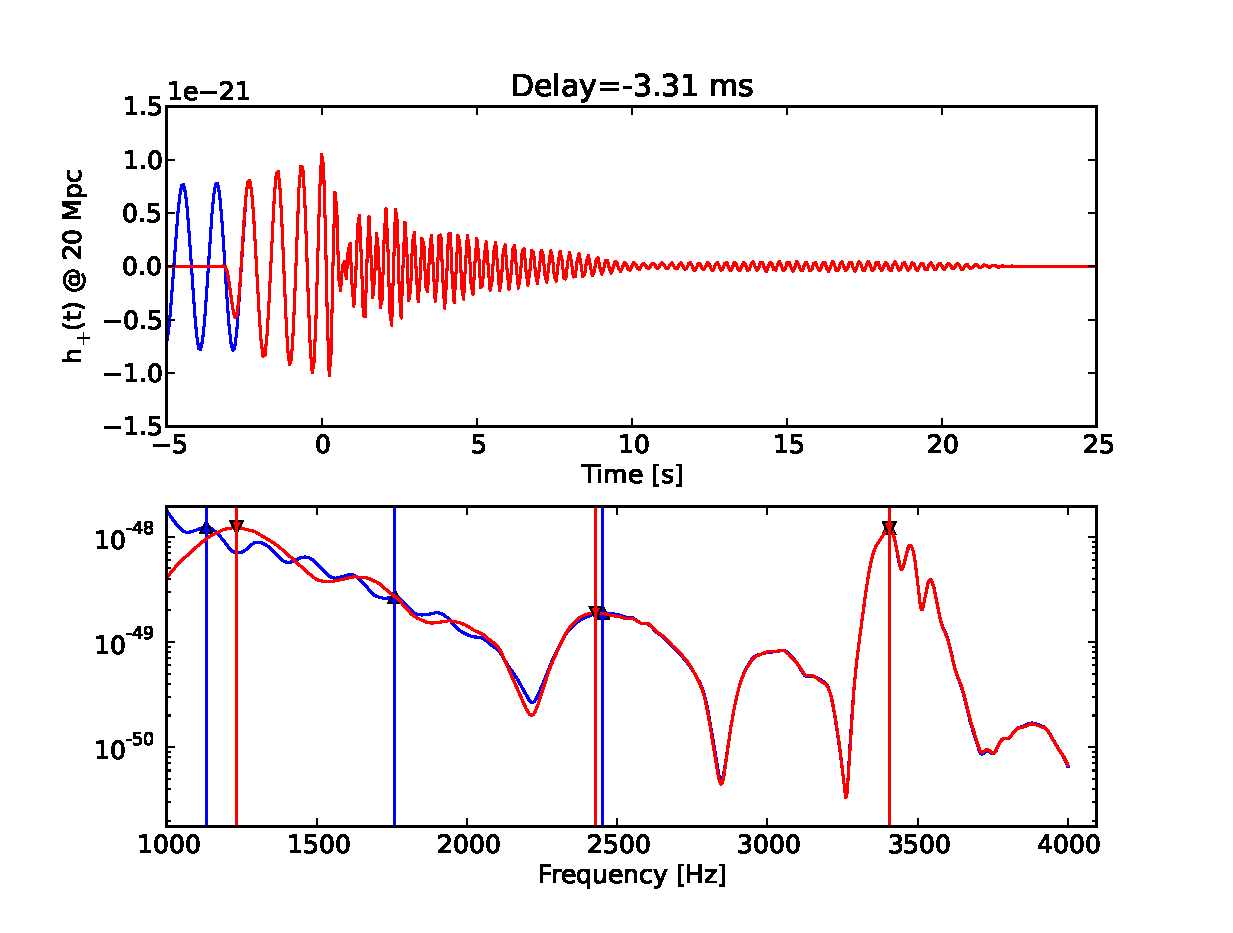
\includegraphics{apr_135135_lessvisc-time_spec--3_31.eps}
            }
        \end{figure}
        \end{center}

        \column{0.5\textwidth}
        \begin{center}
        \begin{figure}
            %\vspace*{-0.5cm}
            \scalebox{0.25}{
            \includegraphics{apr_135135_lessvisc-time_spec--1_65.eps}
            }
        \end{figure}
        \vspace{-0.5cm}
        \begin{figure}
            \scalebox{0.25}{
            \includegraphics{apr_135135_lessvisc-time_spec-0_00.eps}
            }
        \end{figure}
        \end{center}
    \end{columns}

\end{frame}

\begin{frame}
    \frametitle{apr: 1.35-1.35: Time series / spectra: peak trends}

    \begin{center}
        \begin{figure}
            \scalebox{0.5}{
                \includegraphics{apr_135135_lessvisc_peakfreqs.eps}
            }
        \end{figure}
    \end{center}
\end{frame}

%
% DD2 1.35, 1.35
%
\begin{frame}
    \frametitle{DD2: 1.35-1.35: Time series / spectra}

    \begin{columns}[]
        \column{0.5\textwidth}
        \begin{center}
        \begin{figure}
            \scalebox{0.25}{
            \includegraphics{dd2_135135_lessvisc-time_spec--3_82.eps}
            }
        \end{figure}
        \vspace{-0.5cm}
        \begin{figure}
            \scalebox{0.25}{
            \includegraphics{dd2_135135_lessvisc-time_spec--2_55.eps}
            }
        \end{figure}
        \end{center}

        \column{0.5\textwidth}
        \begin{center}
        \begin{figure}
            %\vspace*{-0.5cm}
            \scalebox{0.25}{
            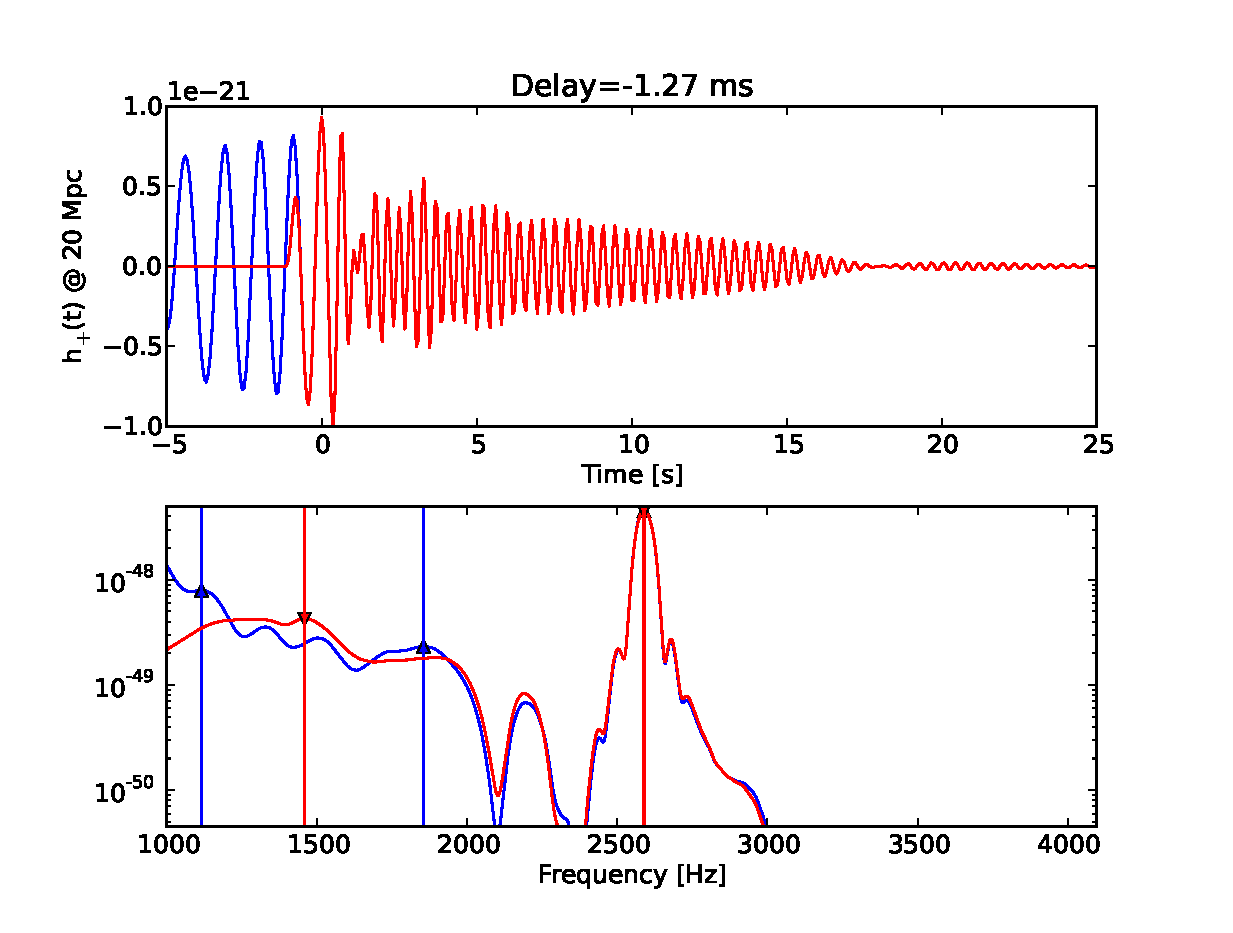
\includegraphics{dd2_135135_lessvisc-time_spec--1_27.eps}
            }
        \end{figure}
        \vspace{-0.5cm}
        \begin{figure}
            \scalebox{0.25}{
            \includegraphics{dd2_135135_lessvisc-time_spec-0_00.eps}
            }
        \end{figure}
        \end{center}
    \end{columns}

\end{frame}

\begin{frame}
    \frametitle{dd2: 1.35-1.35: Time series / spectra: peak trends}

    \begin{center}
        \begin{figure}
            \scalebox{0.5}{
                \includegraphics{dd2_135135_lessvisc_peakfreqs.eps}
            }
        \end{figure}
    \end{center}
\end{frame}

%
% DD2 1.65, 1.65
%
\begin{frame}
    \frametitle{DD2: 1.65-1.65: Time series / spectra}

    \begin{columns}[]
        \column{0.5\textwidth}
        \begin{center}
        \begin{figure}
            \scalebox{0.25}{
            \includegraphics{dd2_165165_lessvisc-time_spec--3_36.eps}
            }
        \end{figure}
        \vspace{-0.5cm}
        \begin{figure}
            \scalebox{0.25}{
            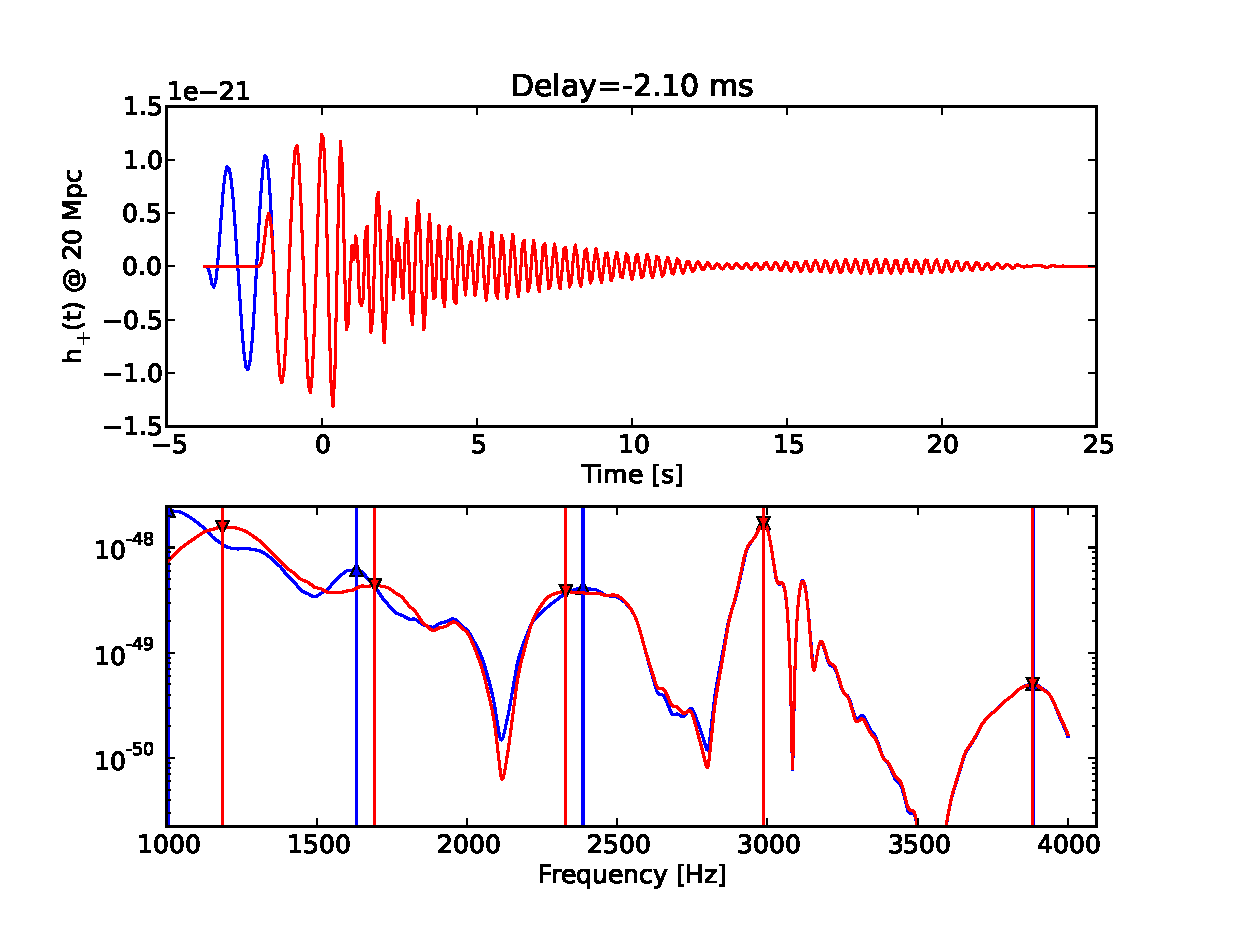
\includegraphics{dd2_165165_lessvisc-time_spec--2_10.eps}
            }
        \end{figure}
        \end{center}

        \column{0.5\textwidth}
        \begin{center}
        \begin{figure}
            %\vspace*{-0.5cm}
            \scalebox{0.25}{
            \includegraphics{dd2_165165_lessvisc-time_spec--0_84.eps}
            }
        \end{figure}
        \vspace{-0.5cm}
        \begin{figure}
            \scalebox{0.25}{
            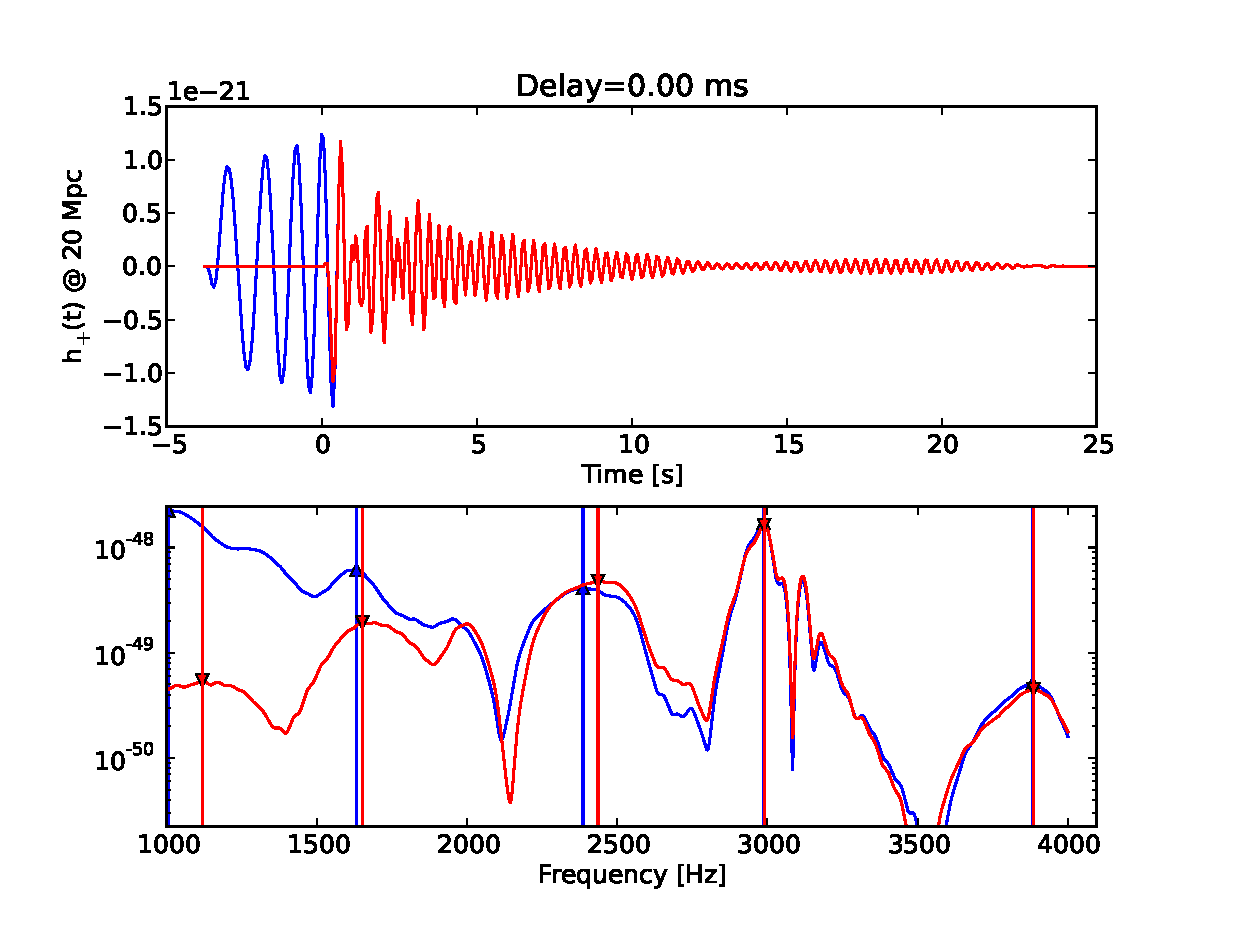
\includegraphics{dd2_165165_lessvisc-time_spec-0_00.eps}
            }
        \end{figure}
        \end{center}
    \end{columns}

\end{frame}

\begin{frame}
    \frametitle{DD2: 1.65-1.65: Time series / spectra: peak trends}

    \begin{center}
        \begin{figure}
            \scalebox{0.5}{
                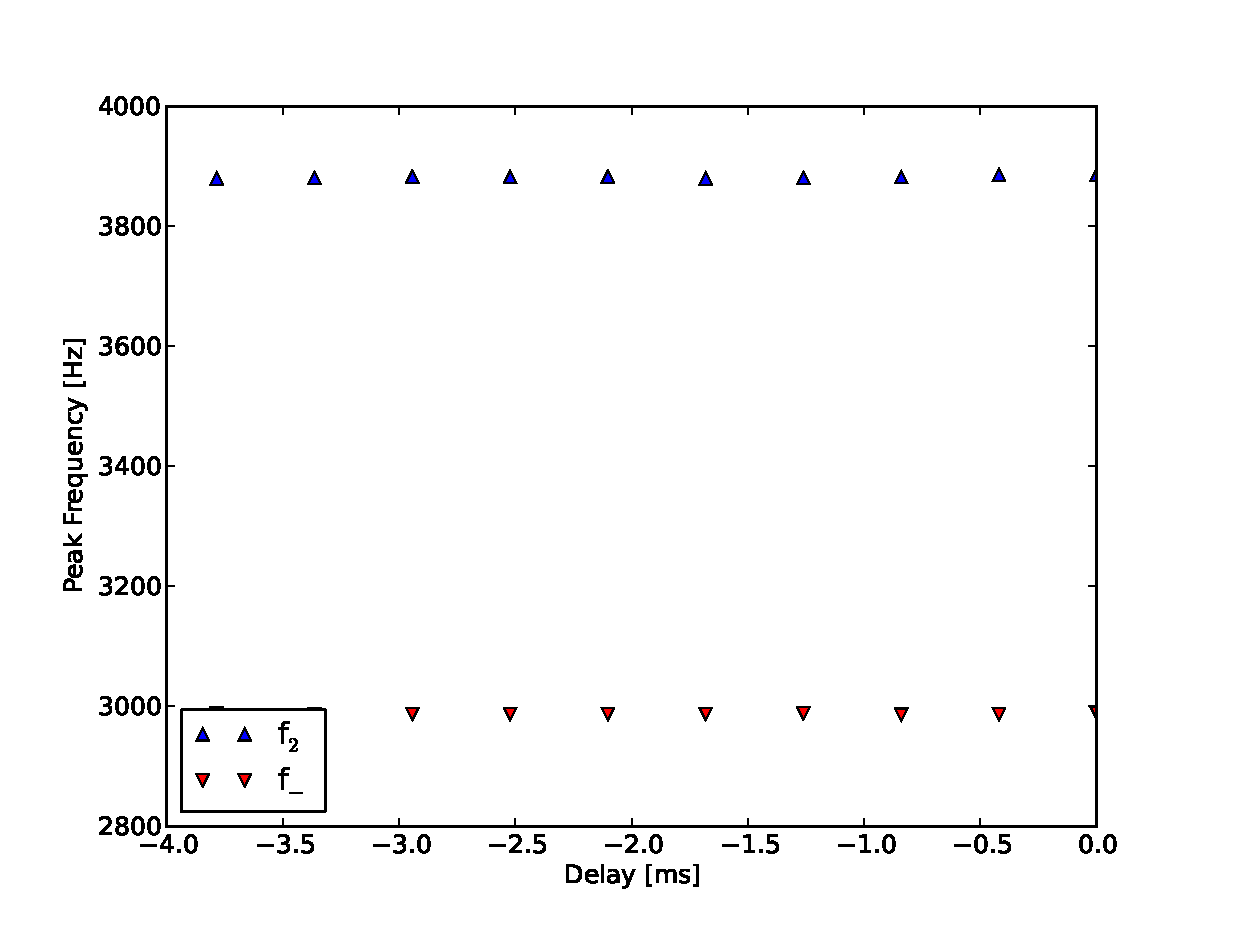
\includegraphics{dd2_165165_lessvisc_peakfreqs.eps}
            }
        \end{figure}
    \end{center}
\end{frame}

%
% NL3 1.35, 1.35
%
\begin{frame}
    \frametitle{NL3: 1.35-1.35: Time series / spectra}

    \begin{columns}[]
        \column{0.5\textwidth}
        \begin{center}
        \begin{figure}
            \scalebox{0.25}{
            \includegraphics{nl3_135135_lessvisc-time_spec--3_26.eps}
            }
        \end{figure}
        \vspace{-0.5cm}
        \begin{figure}
            \scalebox{0.25}{
            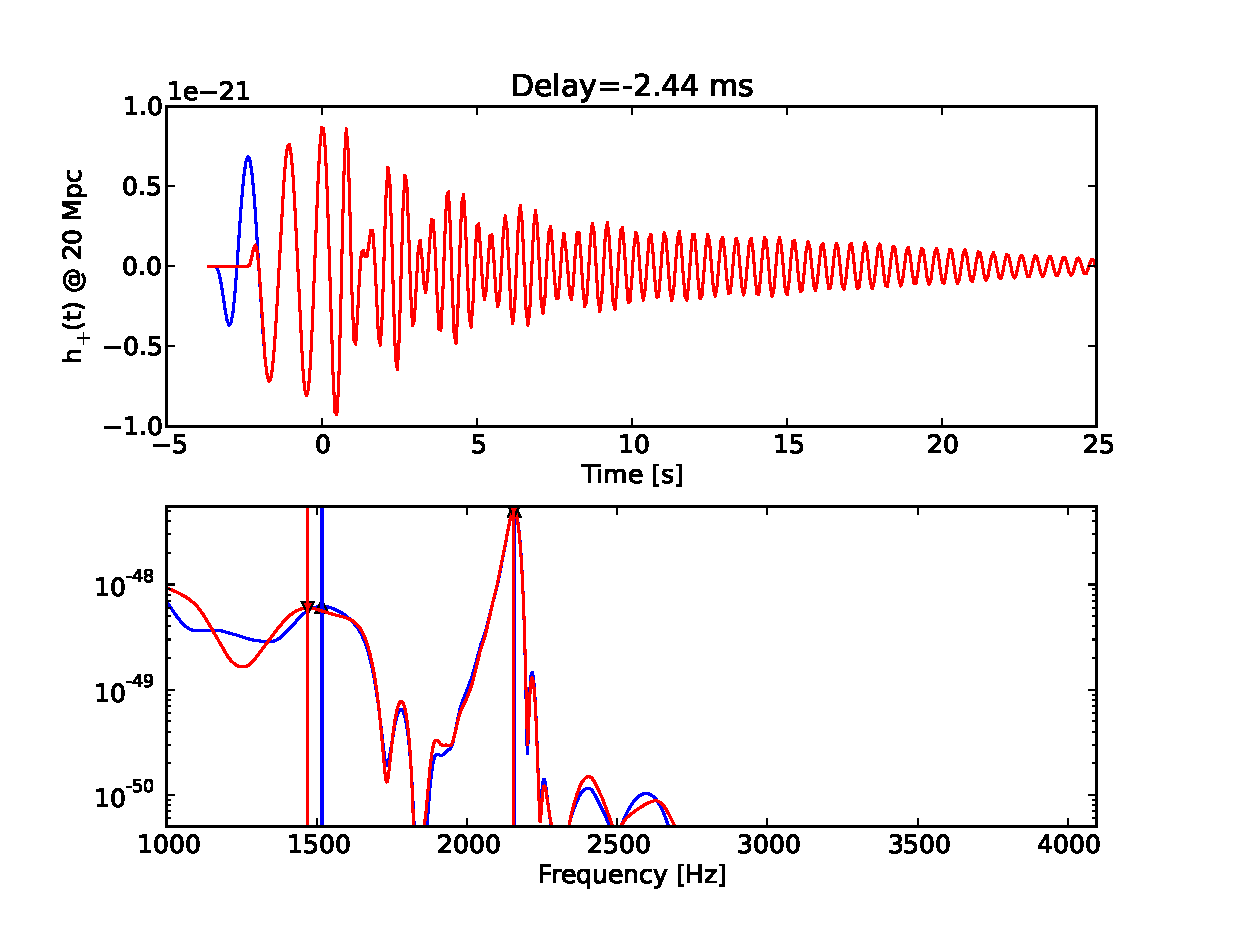
\includegraphics{nl3_135135_lessvisc-time_spec--2_44.eps}
            }
        \end{figure}
        \end{center}

        \column{0.5\textwidth}
        \begin{center}
        \begin{figure}
            %\vspace*{-0.5cm}
            \scalebox{0.25}{
            \includegraphics{nl3_135135_lessvisc-time_spec--0_81.eps}
            }
        \end{figure}
        \vspace{-0.5cm}
        \begin{figure}
            \scalebox{0.25}{
            \includegraphics{nl3_135135_lessvisc-time_spec-0_00.eps}
            }
        \end{figure}
        \end{center}
    \end{columns}

\end{frame}

\begin{frame}
    \frametitle{NL3: 1.35-1.35: Time series / spectra: peak trends}

    \begin{center}
        \begin{figure}
            \scalebox{0.5}{
                \includegraphics{nl3_135135_lessvisc_peakfreqs.eps}
            }
        \end{figure}
    \end{center}
\end{frame}

\begin{comment}
%
% NL3 1.9, 1.9
%
\begin{frame}
    \frametitle{NL3: 1.9-1.9: Time series / spectra}

    \begin{columns}[]
        \column{0.5\textwidth}
        \begin{center}
        \begin{figure}
            \scalebox{0.25}{
            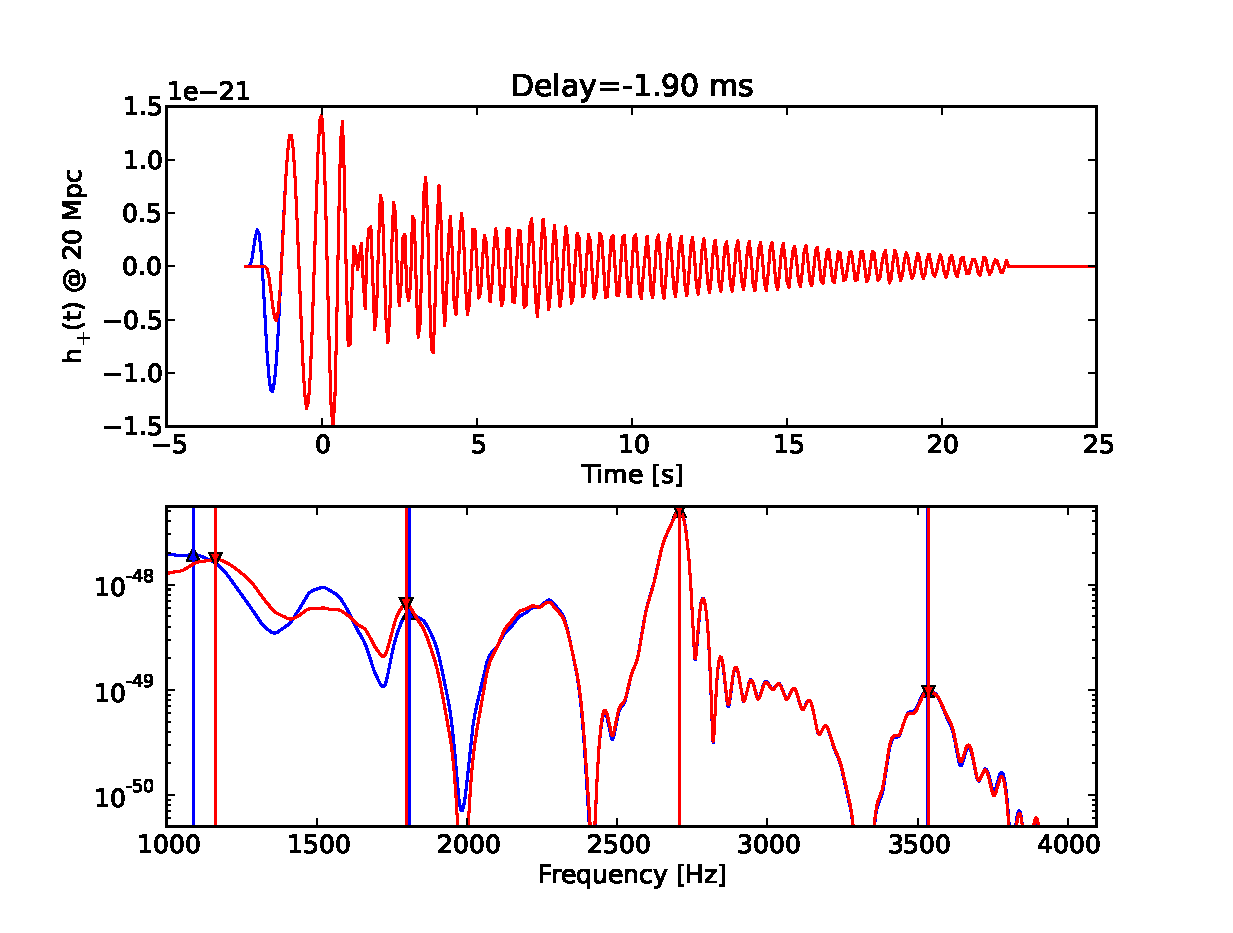
\includegraphics{nl3_1919_lessvisc-time_spec--1_90.eps}
            }
        \end{figure}
        \vspace{-0.5cm}
        \begin{figure}
            \scalebox{0.25}{
            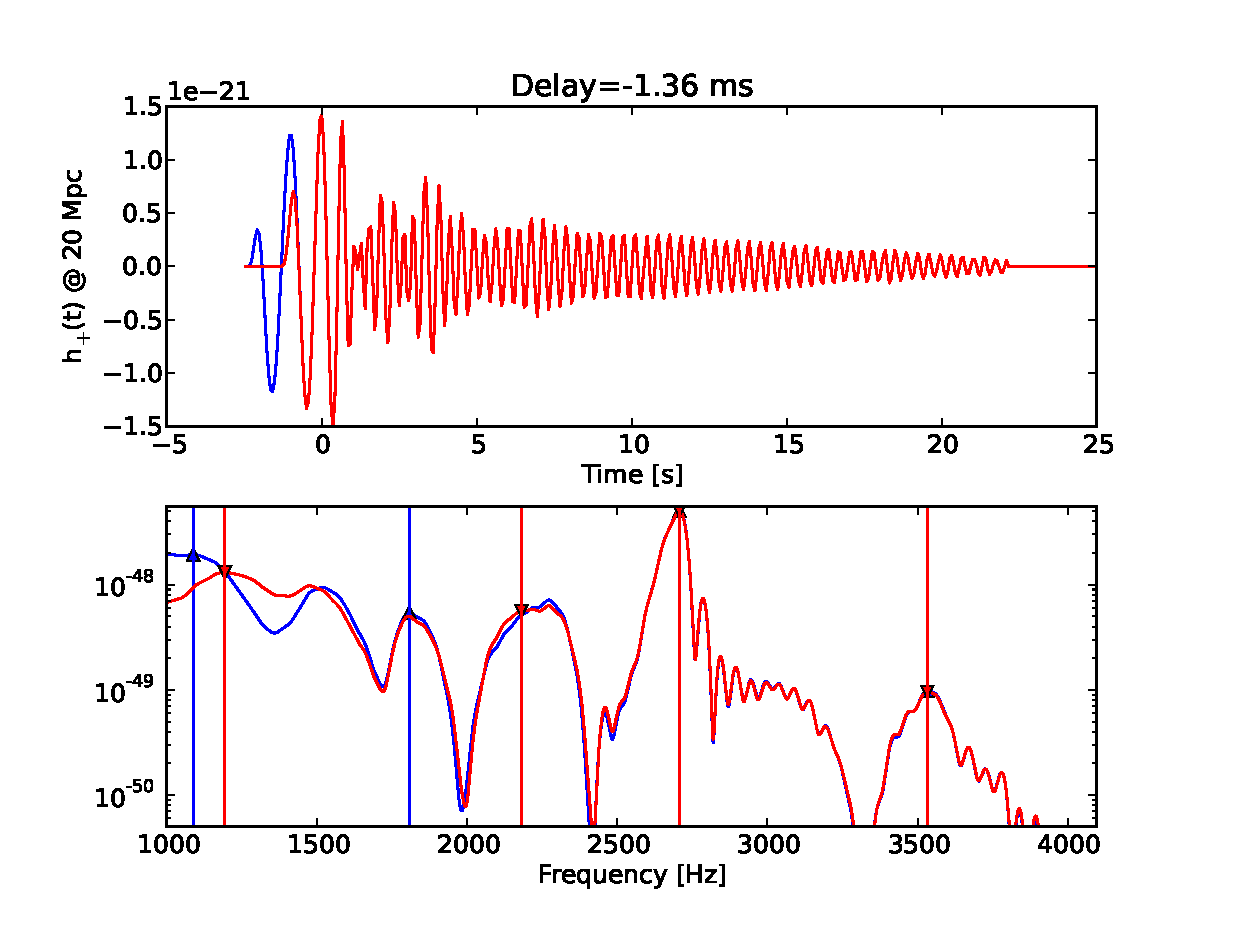
\includegraphics{nl3_1919_lessvisc-time_spec--1_36.eps}
            }
        \end{figure}
        \end{center}

        \column{0.5\textwidth}
        \begin{center}
        \begin{figure}
            %\vspace*{-0.5cm}
            \scalebox{0.25}{
            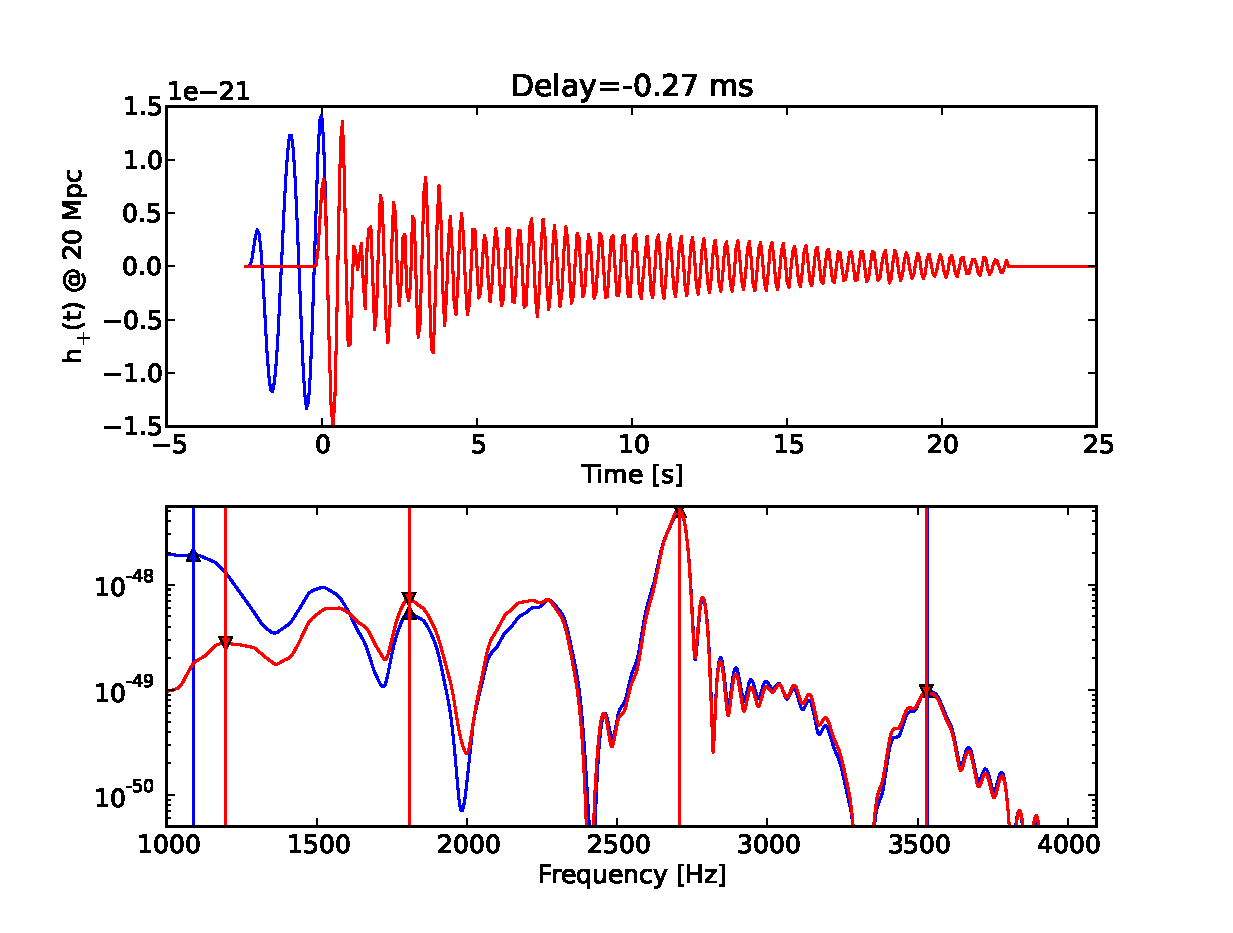
\includegraphics{nl3_1919_lessvisc-time_spec--0_27.eps}
            }
        \end{figure}
        \vspace{-0.5cm}
        \begin{figure}
            \scalebox{0.25}{
            \includegraphics{nl3_1919_lessvisc-time_spec-0_00.eps}
            }
        \end{figure}
        \end{center}
    \end{columns}

\end{frame}
\end{comment}

\begin{frame}
    \frametitle{Plans / on-going}
    \begin{enumerate}
        \item Compute sine-Gaussian match vs delay to demonstrate utility of
            sine-Gaussian parameter estimation for $f_{\text{peak}}$ measurement
        \item Limited Monte-Carlo study of SG parameter estimation with no delay
            using {\tt LALInference} \& example post-merger waveforms to
            highlight necessity of waveform conditioning (or alternative
            templates)
        \item Use burst reconstruction algorithm (CWB) to measure
            $t_{\text{peak}}$ and assess feasibility of truncation
        \item Repeat 1. with waveforms truncated according to $t_{\text{peak}}$
            measurement from CWB
    \end{enumerate}

\end{frame}


\end{document}

